
%(BEGIN_QUESTION)
% Copyright 2012, Tony R. Kuphaldt, released under the Creative Commons Attribution License (v 1.0)
% This means you may do almost anything with this work of mine, so long as you give me proper credit

Build a simple circuit using a battery as the power source, and at least two resistive loads, using a multimeter to correctly measure either voltage or current at specified points in the circuit.  This exercise tests your ability to properly use a multimeter.

$$\includegraphics[width=15.5cm]{i01930x01.eps}$$

\vskip 10pt

The following components and materials will be available to you during the exam: assorted {\bf resistors} ; {\bf terminal strips} ; lengths of {\bf hook-up wire} ; {\bf battery clips} (holders) and {\bf batteries}; {\bf simple multimeters}.

\vskip 10pt

You will be expected to supply your own screwdrivers and digital multimeter (DMM) for assembling and testing the circuit at your desk.  The instructor will supply the battery(ies) to power your circuit when you are ready to see if it works.  Until that time, your circuit will remain unpowered.

\vskip 10pt

\noindent
{\bf Meter measurement} (instructor chooses): \hskip 20pt \underbar{\hskip 20pt} Voltage \hskip 20pt \underbar{\hskip 20pt} Current

\vskip 10pt

\noindent
{\bf Component} (instructor chooses): 

\vfil

\underbar{file i03776}
%(END_QUESTION)





%(BEGIN_ANSWER)


%(END_ANSWER)





%(BEGIN_NOTES)


%INDEX% Mastery exam performance exercise (circuit), measuring DC voltage or current

%(END_NOTES)


